\section{Rik and Andy go to Plop (an abject
Failure)}

\margininbox{Plopzilla}{
     \begin{itemize}
    \item Richard Venn
    \item Andy Jurd
    \end{itemize}}{\explo}

\textit{Written by Rik in a van on the way back across Europe, later typed up by Jarv.}\\

The mission was simple - venture into \passage{Sistem Migovec}, traverse the gaping
holes on \passage{Level 2} to reach the ratty old rope for \passage{Faulty Towers}
and push into \passage{NCB}. Once there we hoped to bottom the fabled
`\passage{Plop}', a big pitch just off \passage{NCB}, rumoured to be over 50 m,
strongly draughting and utterly jinxed!

Armed only with a vague description from a rather drunken Tetley the
night before, we set off for \passage{M16} during a brief lull in the
raging storm. Once down in the cave we quickly hopped up to \passage{NCB},
reviewing the excellent tourist trip across the big stuff in the system.

When we got to \passage{NCB}, we stumbled as \bignote{Tetley had not mentioned the
lairy traverse} over a \textasciitilde{}20 m drop on tatty 13-year-old 9
mm. We concluded that \passage{Plop} was the pitch immediately below the rope from
\passage{Torn T}. This was the error which cost us the pitch. The bolts continued
down the pitch and I had a sinking feeling as I reached the bottom of
this pointless lead.

After this we inspected the rest of \passage{NCB} going East, crossing the
bad traverse with some care. Andy and I took it in turns to examine the
side passages and one of the ones I inspected was, as in the legend of
'95, a very windy squeeze, which could be depth tested by throwing rocks
with some difficulty. I was sure this was it, but Andy had an earlier
memory which led us to think that it might be \passage{Godzilla}. Stones took
around three or four seconds to drop!

We left with five hours to spare before callout, on the very cautious
side, and left the tackle bags at \passage{NCB}. Tomorrow we're going back,
and this time \passage{Plop} must be conquered!

\name{Richard Venn}



\section{The Eventful Conquest of Plopzilla}

\margininbox{Plopzilla}{
     \begin{itemize}
    \item Richard Venn
    \item Andy Jurd
    \end{itemize}}{\explo}

After my first trip to \passage{NCB} I was kept awake thinking about that
three to four second drop known simply as `\passage{Plop}'. By eleven the next
morning I'd managed to convince Andy of the merit of a return visit.
Since we'd left the necessary tools and rope for bolting a monster pitch in \passage{NCB}, we quickly shot down the \passage{M16} entrance series and
up \passage{Faulty Towers} into \passage{NCB}.

Fairly terrified of getting stuck in the tight pitch head above that
formidable drop, I took off most of my SRT kit, leaving just cows-tails
and Croll. The squeeze was fairly easy and Andy passed through the bags as I put in a bolt to make a Y-hang.

Since \passage{Plop} had already been attempted several times there were quite a few existing bolts. I made use of these on the way, stopping only to take down a couple of boost bars: \bignote{a bit of Cadbury Courage}. I felt oddly calm swinging about in the huge chamber. We had thrown more rocks from the top but the bottom was too far away to see. Even from the first rebelay I was having trouble speaking to Andy. Our words boomed around the huge pitch. Two rebelays down, \bignote{I was standing on a gravel floor, shivering with the adrenaline}. I'd been forced to put in a knot pass in the rope and reverse prussic past it. Two more bolts got us to the bottom of the pitch, by which point our nerves were totally shredded.
Though the hang of the rope was very clean, a rope disappearing into
empty blackness above can be really terrifying!

Though we were almost expecting to break into `Level 3', an as-yet
undiscovered horizontal passage at least three kilometres long, the
pitch was completed choked with boulders at its lowest point. We scoured
the nooks and crannies before pronouncing the bottom of \passage{Plop} officially
dead.

However, twenty metres back up the gravel slope, another boulder choke
went down, an obvious lead for a return visit but by this stage we were
too tired to push and survey a new cave passage. We left a going lead in
boulders, along with an easy swing into a window halfway down the pitch.

Exit from the cave was difficult due to being tired and thirsty but \bignote{we were in a jubilant mood after a seventy-six metre survey leg!} \passage{Plop} was the biggest pitch either of us had ever seen. As the first to bottom
this monster, we renamed it `\passage{Plopzilla}'. Analysing the survey data back at the bivi, it measured in at an
impressive 105 m of depth.

\name{Richard Venn}

\begin{pagefigure}
      \checkoddpage \ifoddpage \forcerectofloat \else \forceversofloat \fi
      \centering
              \frame{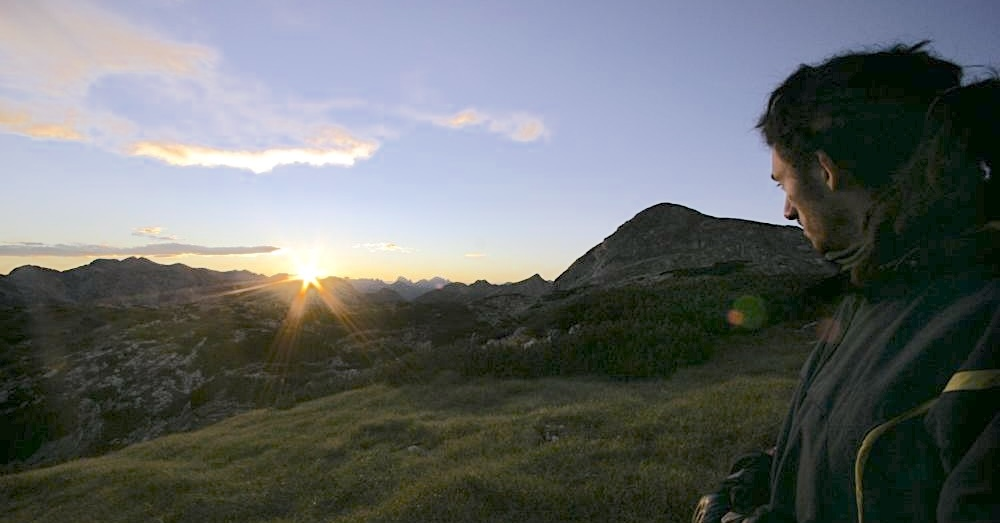
\includegraphics[width=\linewidth]{2007/plop/martin mcgowan -rik watching sunset--orig.jpg}} 
  \caption{Rik watching the setting sun from sunset spot \pic{Martin McGowan}}
\end{pagefigure}
